\chapter{Experiments}\label{ch:experiments}
look at experiment introduction in Grzes phd thesis
\section{\Breakout}



\begin{figure}[h]
	 \centering
	 \begin{subfigure}[b]{0.3\textwidth}
	 	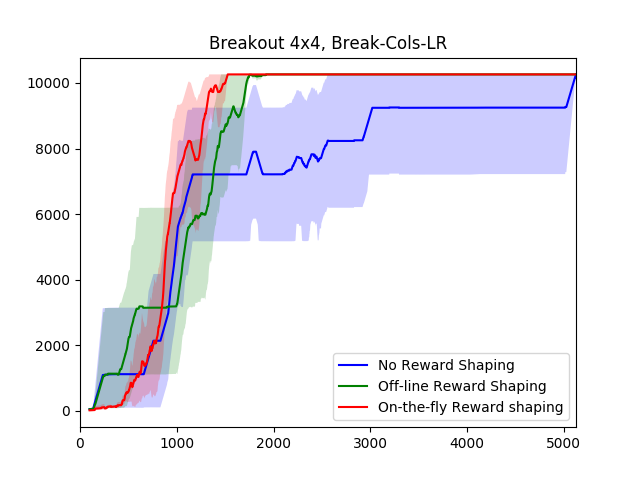
\includegraphics[width=\textwidth]{images/b44-cols-comparison.png}
%	 	\caption{a}
%	 	\label{a}
	 \end{subfigure}
	 ~ %add desired spacing between images, e. g. ~, \quad, \qquad, \hfill etc. 
	 %(or a blank line to force the subfigure onto a new line)
	 \begin{subfigure}[b]{0.3\textwidth}
	 	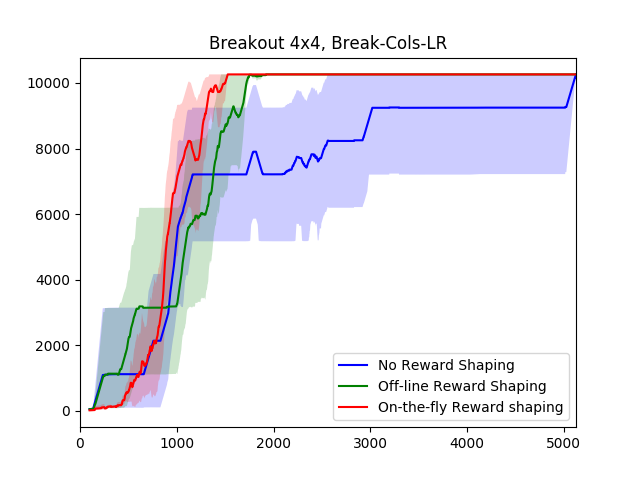
\includegraphics[width=\textwidth]{images/b44-cols-comparison.png}
%	 	\caption{}
%	 	\label{}
	 \end{subfigure}
	 ~ %add desired spacing between images, e. g. ~, \quad, \qquad, \hfill etc. 
	 %(or a blank line to force the subfigure onto a new line)
	 \begin{subfigure}[b]{0.3\textwidth}
	 	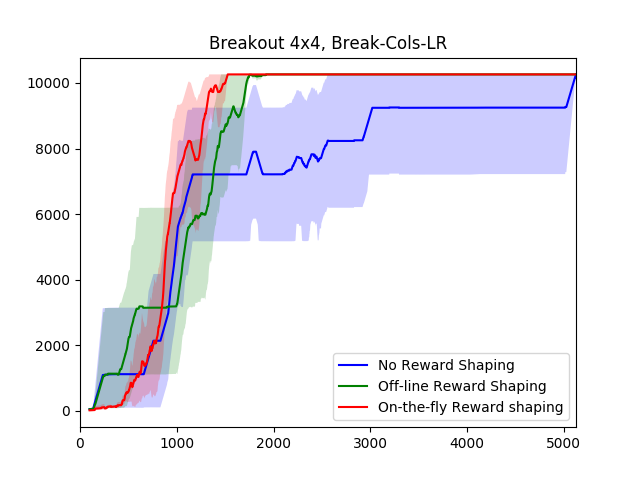
\includegraphics[width=\textwidth]{images/b44-cols-comparison.png}
%	 	\caption{}
%	 	\label{}
	 \end{subfigure}
%	 \caption{}\label{}
\end{figure}

\begin{figure}[h]
	\centering
	\begin{subfigure}[b]{0.3\textwidth}
		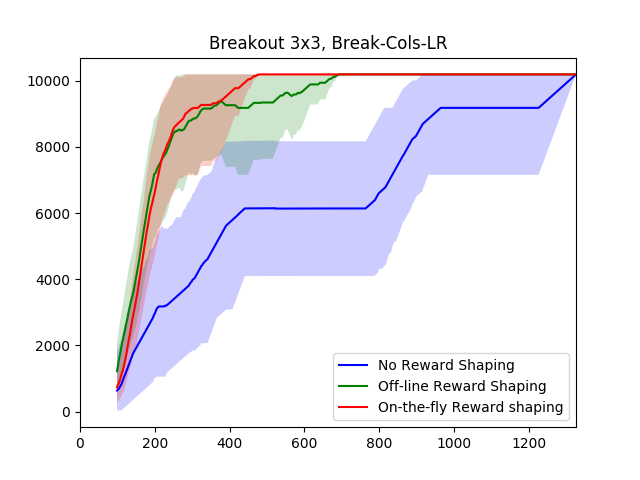
\includegraphics[width=\textwidth]{images/rs-comparison_b33.png}
		%	 	\caption{a}
		%	 	\label{a}
	\end{subfigure}
	~ %add desired spacing between images, e. g. ~, \quad, \qquad, \hfill etc. 
	%(or a blank line to force the subfigure onto a new line)
	\begin{subfigure}[b]{0.3\textwidth}
		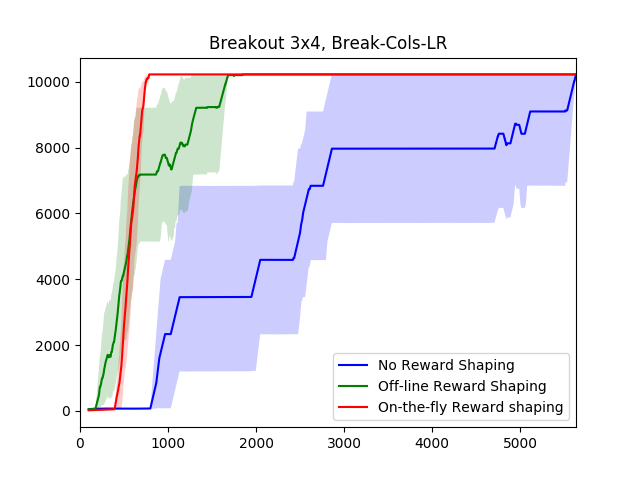
\includegraphics[width=\textwidth]{images/rs-comparison_b34.png}
		%	 	\caption{}
		%	 	\label{}
	\end{subfigure}
	~ %add desired spacing between images, e. g. ~, \quad, \qquad, \hfill etc. 
	%(or a blank line to force the subfigure onto a new line)
	\begin{subfigure}[b]{0.3\textwidth}
		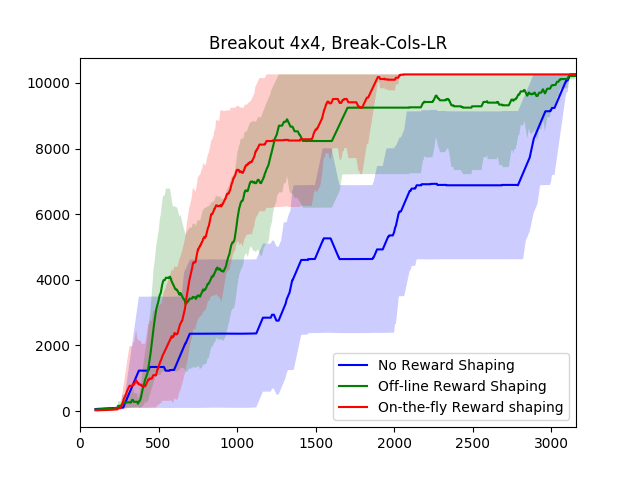
\includegraphics[width=\textwidth]{images/rs-comparison_b44.png}
		%	 	\caption{}
		%	 	\label{}
	\end{subfigure}
	%	 \caption{}\label{}
\end{figure}

\section{\Sapientino}
\section{\Minecraft}